\textbf{Predstavil:} 

Naj bo $f:[0,2] \to \mathbb{R}$ funkcija, katere graf je prikazan na sliki~\ref{fig:trikotniki}. Točke v $x$-os imajo oblike $\left( \frac{1}{2^{i}},0 \right)$ za $i \in \left\{ -1, 0, 1, ... \right\}$, t.j. $(2,0)$, $\left( 1,0 \right)$, $\left( \frac{1}{2},0 \right)$, $\left( \frac{1}{4},0 \right)$, $\left( \frac{1}{8},0 \right)$, ... . Na vsakem intervalu $\left[ \frac{1}{2^{i}}, \frac{1}{2^{i-1}} \right]$ je funkcija $f$ definirana kot linearna naraščajoča funkcija do $x= \frac{3}{2^{i+1}}$, kjer doseže vrednost $1$, t.j. $f\left( \frac{3}{2^{i}} \right) = 1$; torej pa kot padajoča linearna funkcija do točka $x = \frac{1}{2^{i-1}}$, kjer doseže vrednost $0$.

\begin{figure}[h]
	\centering
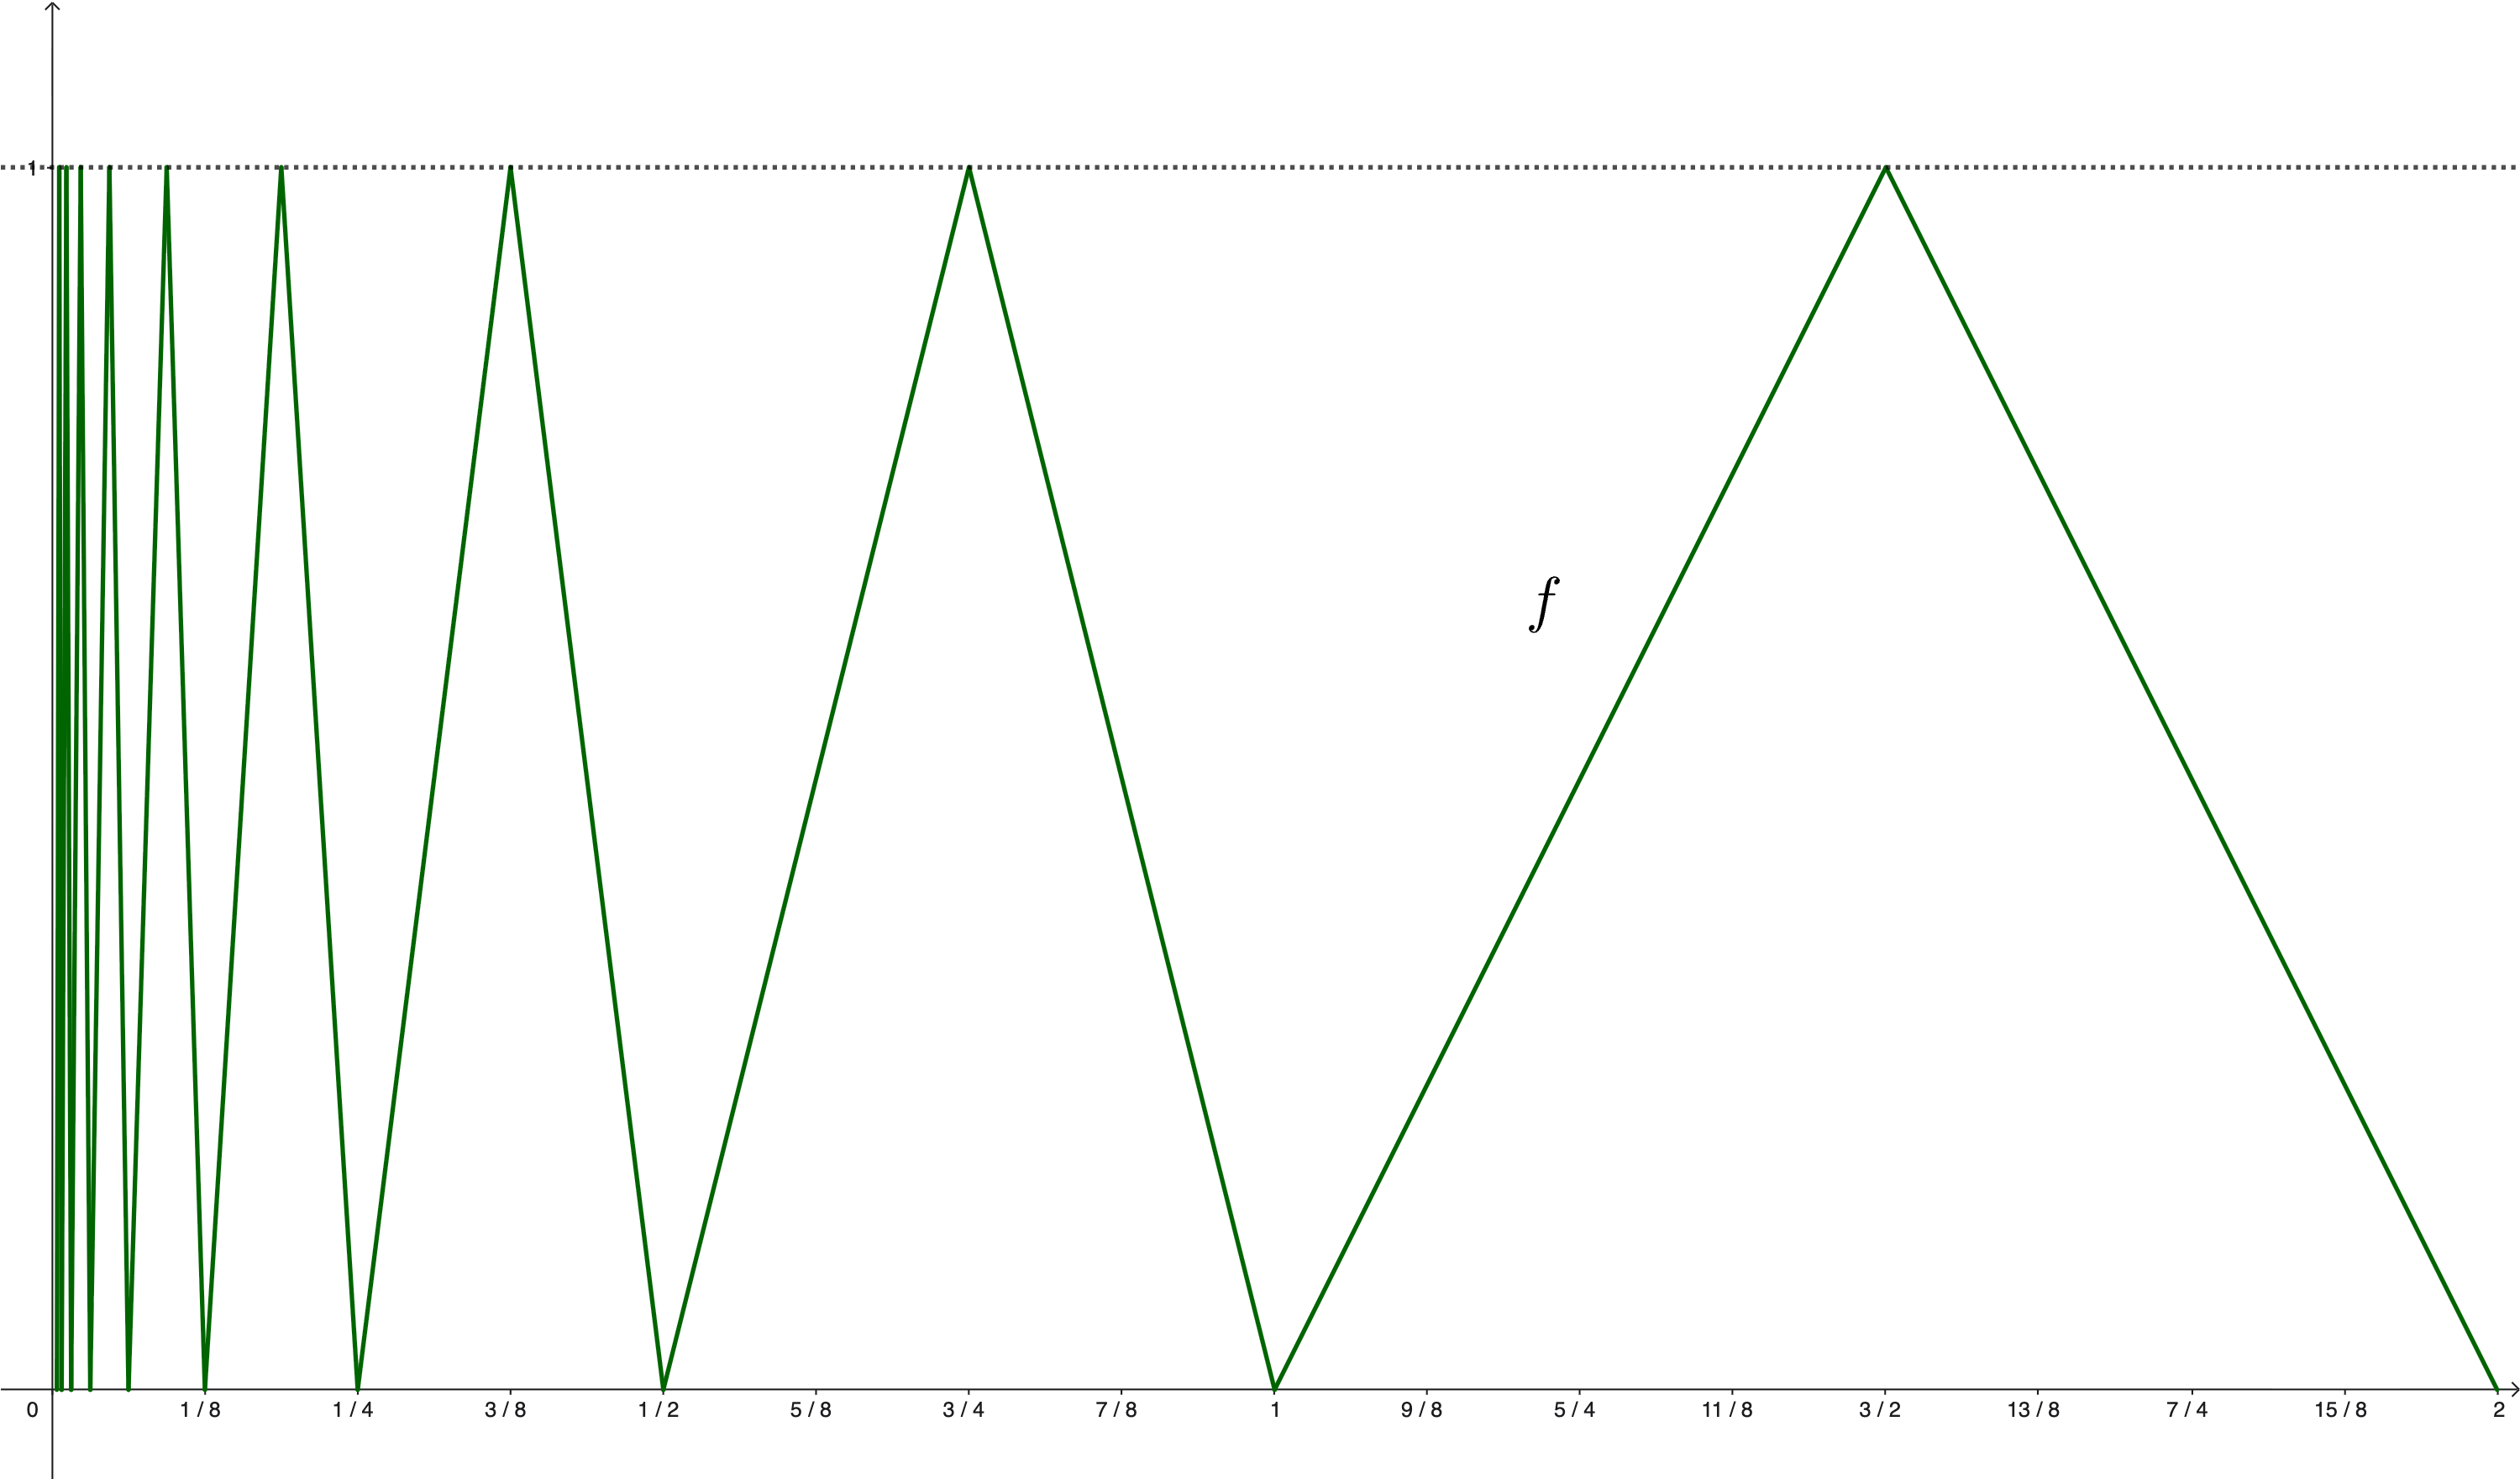
\includegraphics[width=0.5\textwidth]{vaje/graf_trikotniki}
\caption{Graf funkcije $f$.}
\label{fig:trikotniki}
\end{figure}

Določite, ali je funkcija $f$ Riemannovo integrabilna na intervalu $[0,2]$. Če je, izračunajte njen integral $\int_{0}^{2} f(x) dx$.